\documentclass[12pt]{article}


% Math		****************************************************************************************
\usepackage{fancyhdr} 
\usepackage{amsfonts}
\usepackage{amsmath}
\usepackage{amsthm}
\usepackage{dsfont}

% Macros	****************************************************************************************
\usepackage{calc}

% Commands and Custom Variables	********************************************************************
\newcommand{\problem}[1]{\hspace{-4 ex} \large \textbf{#1}\\}
\let\oldemptyset\emptyset
\let\emptyset\varnothing

%page		****************************************************************************************
\usepackage[margin=1in]{geometry}
\usepackage{setspace}
%\doublespacing
\allowdisplaybreaks
\pagestyle{fancy}
\fancyhf{}
\rhead{Shaw \space \thepage}
\setlength\parindent{0pt}

%Code		****************************************************************************************
\usepackage{listings}
\usepackage{courier}
\lstset{
	language=Python,
	showstringspaces=false,
	formfeed=newpage,
	tabsize=4,
	commentstyle=\itshape,
	basicstyle=\ttfamily,
}

%Images		****************************************************************************************
\usepackage{graphicx}
\graphicspath{ {images/} }

%Hyperlinks	****************************************************************************************
%\usepackage{hyperref}
%\hypersetup{
%	colorlinks=true,
%	linkcolor=blue,
%	filecolor=magenta,      
%	urlcolor=cyan,
%}


\begin{document}
	\thispagestyle{empty}
	
	\begin{flushright}
		Sage Shaw \\
		m527 - Fall 2017 \\
		\today
	\end{flushright}
	
{\large \textbf{HW 4}}\bigbreak

\problem{(a)}
	Note that I have assumed the curve is oriented counter-clockwise.\\
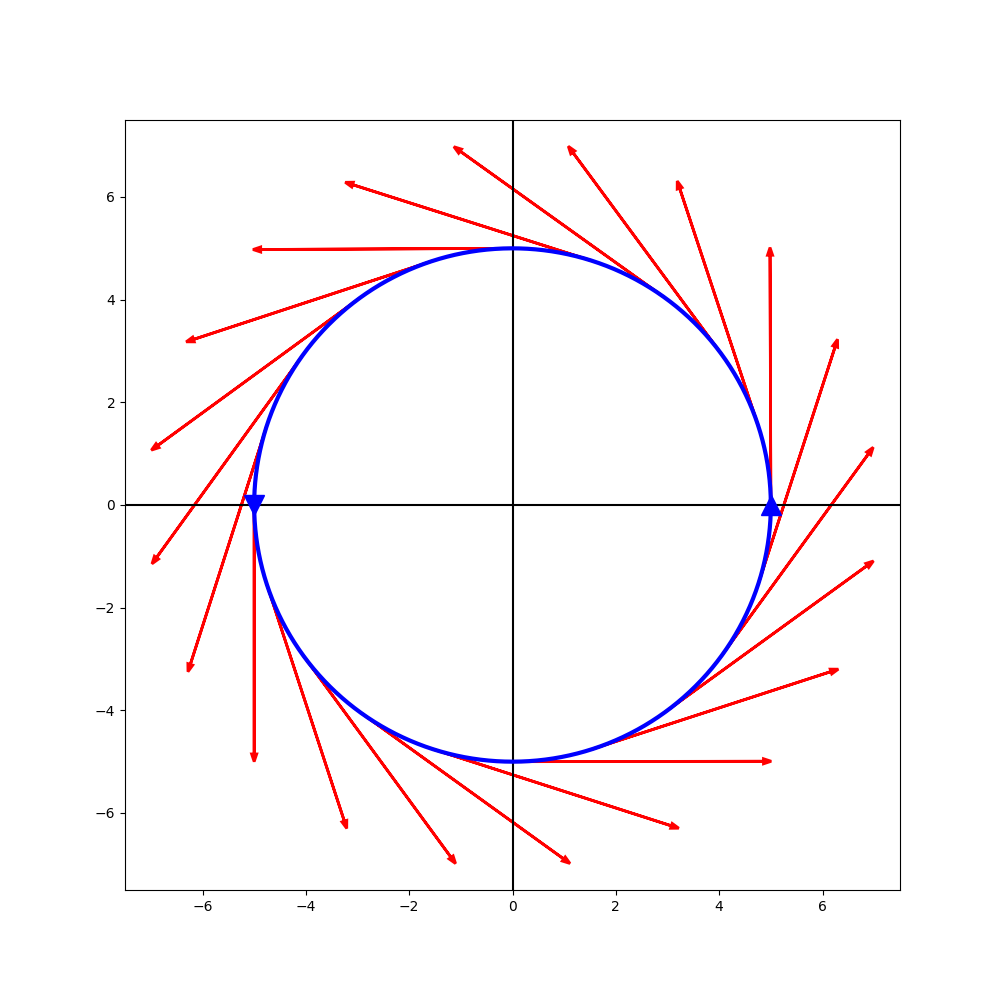
\includegraphics[width=1.0\textwidth]{hw5_figure_1}

\problem{(b)}
	Since the velocity field at each point on the curve is pointing in the direction of the curve, we expect the circulation to be positive.

\problem{(c)}
	Since the velocity field at each point on the curve is tangent to the curve, we expect the flux to be zero.
	
\problem{(d)}
	First note the parametaraization of our curve: $r(t) = [5\text{cos}(t), 5 \text{sin}(t)]^T$ for $0 \leq t \leq 2\pi$.
	Using our equation for circulation where $M(x,y) = -y$ and $N(x,y) = x$ we get
	\begin{align*}
		\text{circ} & = \int_{C}(Mdx + Ndy) \\
		& = \int_{0}^{2\pi} M\big(x(t),y(t)\big)\tfrac{dx}{dt} + N\big(x(t),y(t)\big) \tfrac{dy}{dt} dt \\
		& = \int_{0}^{2\pi} -5 \text{sin}(t)(-5\text{sin}(t)) + 5\text{cos}(t)(5\text{cos}(t)) dt \\
		& = \int_{0}^{2\pi} 25(\sin^2 t+\cos^2 t) dt \\
		& = 25\int_{0}^{2\pi} 1 dt \\
		& = 50\pi
	\end{align*}
	As expected the circulation is positive.\\
	
\problem{(e)}
	With the same parametariziation as above we calculate the flux as follows
	\begin{align*}
		\text{flux} & = \int_{C}(Mdy - Ndx) \\
		& = \int_{0}^{2\pi} M\big(x(t),y(t)\big)\tfrac{dy}{dt} - N\big(x(t),y(t)\big) \tfrac{dx}{dt} dt \\
		& = \int_{0}^{2\pi} -5 \text{sin}(t)(5\text{cos}(t)) - 5\text{cos}(t)(-5\text{sin}(t)) dt \\
		& = \int_{0}^{2\pi} 0 dt \\
		& = 0
	\end{align*}
	The flux is zero as expected.
	
\problem{(f)}
	We will now compute the circulation using Green's Theorem.
	\begin{align*}
		\text{circ} = \int_{C}(Mdx + Ndy) & = \iint_{R}\Big(\frac{\partial N}{\partial x} - \frac{\partial M}{\partial y}\Big) dA \\
		& = \iint_{R}\big(1 - (-1)\big) dA \\
		& = \iint_{R}2 dA \\
		& = 50 \pi
	\end{align*}
	As expected, Green's Theorem gives the same result as our line integral.
	
\problem{(g)}
	We will now compute the flux using Green's Theorem as before. However, this time we will need to change to polar coordinates via the following substitutions: \bigbreak
	\begin{align*}
		x &= r\cos \theta & y &= r\sin \theta \\
		dA &= r dr d\theta&& \\
		\text{where } 0 & \leq r \leq 5 & \text{and } 0 &\leq \theta \leq 2\pi
	\end{align*} \bigbreak
	We calculate flux like so
	\begin{align*}
		\text{flux} = \int_{C}(Mdy - Ndx) & = \iint_{R}\Big(\frac{\partial M}{\partial x} + \frac{\partial N}{\partial y}\Big) dA \\
		& = \iint_{R}-y + x dA \\
		& = \int_{0}^{2\pi} \int_{0}^{5} (-\sin \theta + cos \theta) r dr d\theta \\
		& = \int_{0}^{2\pi} (-\sin \theta + cos \theta)\int_{0}^{5} r dr d\theta \\
		& = \int_{0}^{2\pi} (-\sin \theta + cos \theta)\Bigg( \tfrac{1}{2}r^2 \Big\vert_{0}^{5}\Bigg) d\theta \\
		& = \int_{0}^{2\pi} (-\sin \theta + cos \theta)\tfrac{25}{2} d\theta \\
		& = \tfrac{25}{2} \Bigg( cos \theta + \sin(\theta)\Big\vert_{0}^{2\pi}\Bigg) \\
		& = 0
	\end{align*}
	As expected, Green's Theorem gives the same result as our line integral.
	
\end{document}
